\documentclass{article}

\usepackage[left=2cm,right=2cm, top=2cm, bottom = 2cm]{geometry}
\usepackage{amsfonts}


\usepackage{amsmath}
\usepackage{xcolor}

\usepackage{tikz}
\usepackage{subfigure}




\pagestyle{empty}

\setlength{\tabcolsep}{15pt}

\newcommand{\deriv}[3][]{\frac{\mathrm{d}^{#1}#2}{\mathrm{d}#3^{#1}}}
\newcommand{\diff}{\;\mathrm{d}}


\begin{document}

\title{Numerical Solution of ODEs}
\date{}

\maketitle
\thispagestyle{empty}

\Large

\textbf{\underline{Objective: To be familiar with and able to use Euler's Method and}}

\textbf{\underline{the classical Runge-Kutta Method to solve ODEs.}}







\vspace{5mm}











\textbf{Recap: Integrating Factors:}\bigskip


A resistor heats up to a temperature of $80^\circ\mathrm{C}$. It is connected to a heat sink at the ambient temperature of $20^\circ\mathrm{C}$; we will assume the heat capacity of the heat sink is high enough that it does not heat up appreciably as it dissipates the heat from the resistor.

Let $\theta(t)$ be the temperature of the resistor, starting from time $t=0$, when it is at $80^\circ\mathrm{C}$ and no further heating is applied. Newton's Law of Cooling says that the rate at which the temperature decreases is proportional to the difference in temperature between the resistor and the heat sink; as an ODE:
\[\deriv{\theta}{t} = k(20-\theta),\]
where $k$ is a positive constant measuring how efficiently heat is conducted from the resistor into the heat sink. Rewriting this, and supposing $k=5$, we have
\[\deriv{\theta}{t}+5\theta = 100.\]

Solve this equation by an integrating factor and use the initial conditions from the setup to find the time at which the resistor temperature drops below $30^\circ\mathrm{C}$.\bigskip



Note: this ODE can also be solved by separation of variables. For extra practice at separation of variables, check that this gives the same solution as the integrating factor method!






\clearpage









\textbf{Warm-up: Euler's Method:}\bigskip

Consider the initial value problem
\[\deriv{x}{t} = 2x,\qquad x(0)=1.\]

We can solve this analytically by separation of variables---the solution is $x=e^{2t}$. We shall look at how, even if we didn't know the solution, we can estimate the value of a solution at a given time. The exact solution at time 1 is $x(1)=e^2\approx7.3890561$. We will see how to estimate this from the equation, without using any knowledge of the solution. The idea is to use the first-order Taylor polynomial of the solution:
\[x(t)\approx x(0) + x'(0)t.\]
The smaller the value of $t$, the more accurate this estimate is.

\begin{enumerate}
	\item Use the ODE and initial condition to find the value of $x'(0)$, and hence write down the first-order Taylor polynomial of $x(t)$ about $t=0$.
	\item Use the Taylor polynomial to estimate $x(1)$.
	\item The estimate above is not very accurate, because we aren't taking many terms in the Taylor series, and aren't very close to the basepoint of the series. We can get a more accurate estimate as follows:
		\begin{enumerate}
			\item First use the Taylor polynomial about $t=0$ to estimate the value of $x(0.5)$.
			\item Now use the original ODE and your estimate of $x(0.5)$ to estimate $x'(0.5)$.
			\item Hence write down the first-order Taylor polynomial of $x(t)$ about $t=0.5$.
			\item Use this Taylor polynomial to estimate $x(1)$.
		\end{enumerate}
	\item Now find a still more accurate estimate of $x(1)$ by first estimating $x(0.2)$, then finding the Taylor expansion about $t=0.2$, using it to estimate $x(0.4)$, then using this to Taylor expand about $t=0.4$ and so on.
\end{enumerate}









\clearpage














\textbf{Theory: Euler's Method:}

\bigskip

Suppose we have an initial value problem
\[\deriv{x}{t}=f(t,x),\qquad x(0)=x_0,\]
for some known function $f$. Depending on what $f$ is, we might be able to solve this by separation of variables or an integrating factor, and these methods do work for several equations that arise in real-world problems. However, for many problems, neither of these methods works. Often, the best we can do is to estimate values of the solution at different times.

The most straightforward way to do this is Euler's Method, which we saw in the warm-up. The idea is to treat the solution as ``locally linear''---\textit{i.e.}, to approximate it by a sequence of short straight lines. Take a small increment of time $h$ (called the \textbf{timestep} or \textbf{step-size}). We start with $x_0$, the initial condition, and use the ODE to see that $x'(0)=f(0,x_0)$; then $x(h)\approx x(0)+hx'(0)=x_0+hf(0,x_0)$. So we set $x_1=x_0+hf(0,x_0)$, and treat this as our estimate of $x(h)$.

We can then iterate this; in general, if we have $x_n\approx x(t_n)$, then the ODE gives $x'(t_n)=f(t_n,x(t_n))\approx f(t_n,x_n)$, and $x(t_n+h)\approx x(t_n)+hf(t_n,x_n)$; we take this to be $x_{n+1}$, our estimate of $x(t_{n+1})$, where $t_{n+1}=t_n+h$. We have the iterative formula
\[x_{n+1}=x_n+hf(t_n,x_n).\]

The smaller the step-size, the more accurate the estimate is likely to be. Nonetheless, the estimate becomes less and less accurate as $n$ grows larger---each estimate is based on the previous estimates, so errors accumulate. This is a characteristic of all numerical methods for solving ODEs---the further into the future you want to estimate the solution, the less accurate your estimate is likely to be.

We illustrate Euler's Method overleaf with the equation $x'=x$ and the initial condition $x(0)=1$; the exact solution is $x=e^t$.



\begin{center}
\begin{tikzpicture}
	\draw[->] (0,0) -- (12,0);
	\node[right] at (12,0) {$t$};
	\draw[->] (0,0) -- (0,20);
	\node[above] at (0,20) {$x$};
	
	\foreach \i in {0,1,2,3}{
		\node[below] at ({4*\i},0) {\i};
	}
	
	\foreach \i in {0,1,...,20}{
		\node[left] at (0,\i) {\i};
	}
	
	\draw[thick,blue,domain=0:12,samples=100] plot (\x,{ exp(\x/4) });
	
	\draw[thick,cyan] (0,1) -- (6,2.5) -- (12,6.75);
	
	\draw[thick,red] (0,1) -- (4,2) -- (8,4) -- (12,8);
	
	\draw[thick,violet] (0,1) -- (3,1.75) -- (6,3.0625) -- (9,5.359375) -- (12,9.37890625);
	
	\draw[thick,green] (0,1) -- (2,1.5) -- (4,2.25) -- (6,3.375) -- (8,5.0625) -- (10,7.59375) -- (12,11.390625);
	
	\draw[thick,yellow] (0,1) -- (1,1.25) -- (2,1.5625) -- (3,1.953125) -- (4,2.44140625) -- (5,3.0517578125) -- (6,3.81469726563) -- (7,4.76837158204) -- (8,5.96046447755) -- (9,7.45058059694) -- (10,9.31322574618) -- (11,11.6415321827) -- (12,14.5519152284);

	\matrix[draw,below] at (current bounding box.south) {
		\node[blue,left] {$y=e^x$};
		\node[cyan,right] {$h=1.5$};\\
		\node[red,left] {$h=1$};
		\node[violet,right] {$h=0.75$};\\
		\node[green,left] {$h=0.5$};
		\node[yellow,right] {$h=0.25$};\\
	};
\end{tikzpicture}
\end{center}








\clearpage










\textbf{Theory: Runge-Kutta Methods:}

\bigskip


From the graph, we see that the smaller our step-size, the more accurate our approximation, especially at larger times. However, even with the smallest step-size displayed, $h=0.25$, the error quickly becomes fairly large. For each interval, from $t_n$ to $t_{n+1}=t_n+h$, we use our estimate $x_n$ and plug it into the ODE to get an estimate of $x_n$ for the derivative of the solution at $t_n$. We then assume that derivative remains constant from $t_n$ to $t_n+h$; however, the actual solution has derivative that always increases (exponentially!), so the estimate we are using for the derivative all along the interval $t_n$ to $t_n+h$ is actually the minimum value of the derivative over that subinterval - so we're bound to underestimate the value of the solution at $t_{n+1}$. Since each estimate depends on the previous one, this error grows worse and worse, and each successive step underestimates the correct value by a larger amount.

For different initial value problems, we will observe the opposite effect; with the same equation, but the initial condition $x(0)=-1$, the solution is $x(t)=-e^t$, and Euler's method will overestimate the solution at each step. For some initial value problems, Euler's method might sometimes underestimate and sometimes overestimate the solution, and so might manage (essentially by chance) to stay closer to the correct solution; but we can see that, in general, we cannot rely on Euler's method to give us accurate estimates of the solution for large values of $t$, even with a very small step-size. This ultimately comes down to the fact that $x'(t_n)$ is not generally a good estimate of the average rate-of-change between $t_n$ and $t_{n+1}$.

How can we correct this? We want a better estimate of the average rate-of-change from $t_n$ to $t_{n+1}$ than simply $x'(t_n)$ (or, what's worse, our estimate of $x'(t_n)$ based on our previous estimates!). If we could estimate the derivative of the solution at $t_n$ and $t_{n+1}$, we could average these, then use this as the gradient of our straight-line approximation. The problem is how we estimate the derivative at $t_{n+1}$ without already knowing an estimate $x_{n+1}$ of the solution at $t_{n+1}$---which is what we're trying to find, after all.

The idea is to use Euler's method to get a rough estimate of $x_{n+1}$, use this to estimate $x'(t_{n+1})$, then average this with our estimate of $x'(t_n)$ and use this average rate-of-change as the gradient of our straight line. We will illustrate with the same example as we used for Euler's method in the warm-up.






\clearpage





\textbf{Practice/Example:}

\vspace{5mm}

We will again attempt to solve the initial value problem
\[\deriv{x}{t}=2x,\qquad x(0)=1,\]
using the improved method described on the last page.
The correct value of the solution at $t=1$ is $e^2\approx 7.3890561$. Using Euler's method with a step-size of 1, we estimated $x(1)\approx 3$; with a step-size of $0.5$, we had $x(1)\approx 4$, and with a step-size of $0.2$, we had $x(1)\approx 5.38$.

\begin{enumerate}
	\item First we will use a step-size of $0.5$.
		\begin{enumerate}
			\item Use the ODE to find the initial derivative, $x'(0)$; call this $k_1$.
			\item Use this initial derivative to find a working estimate of $x(0.5)$ by Euler's method.
			\item Use this working estimate to estimate $x'(0.5)$; call this $k_2$.
			\item Using the average, $\frac{1}{2}(k_1+k_2)$ as the rate-of-change, find an improved estimate of $x(0.5)$. Call this $x_1$.
			\item Now use $x_1$ to estimate $x'(0.5)$ from the ODE; call this $k_1$ (you can forget the old value of $k_1$!).
			\item Use $y_{1,0}$ as the rate-of-change to find an Euler's method working estimate of $x(1)$.
			\item Use this working estimate to estimate $x'(1)$; call this $k_2$.
			\item Using $\frac{1}{2}(k_1+k_2)$ as the rate-of-change, find an improved estimate of $x(1)$. Call this $x_2$, and compare with the estimate obtained by Euler's method.
		\end{enumerate}
	\item Now repeat the above steps, but with a step-size of $0.1$. Compare this with the estimate obtained by Euler's method.
\end{enumerate}




\clearpage





\textbf{Theory: Runge-Kutta Methods (cont.):}\bigskip


We saw above that by first using Euler's method to find a working estimate of the solution after a time-step, then averaging the estimate of the derivative at the left of the interval with the estimate obtained at the right of the interval from our working estimate of the solution, we can get a significantly more accurate estimate of the solution, even with relatively big step-sizes. This is called a two-step \textbf{Runge-Kutta Method}. Euler's method itself is a one-step Runge-Kutta method.

In general, an $m$-step Runge-Kutta method takes $m$ different estimates of the derivative between $t_n$ and $t_n+h$, then averages these to get an overall estimate for the average rate-of-change across that timestep, which is then used to estimate the solution at $t_n+h$. Often, a weighted average is used when combining the different estimates of the derivative. Typically, the first estimate of the derivative comes from simply plugging $x_n$ into the ODE; this is then used to move for all or part of the timestep to get a working estimate of the solution at a later time, from which we obtain a second estimate of the derivative. Then we use this second estimate to find another estimate of the solution at some point in the timestep, and use this to get a third estimate of the derivative, and so on.

The most common Runge-Kutta method used is called \textbf{the classical fourth-order Runge-Kutta method}, or RK4 for short. It is a 4-step Runge-Kutta method, though this is not what the term ``fourth-order'' refers to: the error in an estimate obtained by RK4 is on the order $h^4$; this means that if you halve the step-size, you expect the error to be reduced by a factor or 16. Five-step Runge-Kutta methods are also fourth-order, which means the extra work of finding a fifth estimate of the derivative to average with the others is not rewarded by a significant increase in accuracy. It is for this reason that RK4 is so widely used---it gives the best accuracy without an unreasonable increase in computational difficulty. A five-step Runge-Kutta method will tend to be more accurate than RK4, but not by enough to justify the increase in computational complexity, whereas RK4 is significantly better than any three-step Runge-Kutta method, so is worth the extra difficulty.


\clearpage



\textbf{The Classical Runge-Kutta Method:}\bigskip


RK4 works as follows for the ODE $x'(t)=f(t,x)$: given $x_n$ an estimate of $x(t_n)$, define
\begin{align*}
	k_1 &= f(t_n,x_n),\quad y_1=x_n+k_1\frac{h}{2}\\
	k_2&=f\left(t_n+\frac{h}{2},y_1\right),\quad y_2=x_n+k_2\frac{h}{2}\\
	k_3&=f\left(t_n+\frac{h}{2},y_2\right),\quad y_3=x_n+k_3h\\
	k_4&=f(t_n+h,y_3).
\end{align*}
Then we set $t_{n+1}=t_n+h$, and
\[x_{n+1}=x_n + \frac{k_1+2k_2+2k_3+k_4}{6}h.\]

So we use $k_1$, which is the estimate of $x'(t_n)$ according to the ODE and $x_n$, to find a working estimate $y_1$ of $x\left(t_n+\frac{h}{2}\right)$; that is, we use Euler's method, but only go half of the timestep, to the middle of the interval $t_n$ to $t_n+h$. Then we use this working estimate $y_1$ to estimate $x'\left(t_n+\frac{h}{2}\right)$, and call this $k_2$; $k_2$ is then used to find $y_2$, a second estimate of $x\left(t_n+\frac{h}{2}\right)$. We then plug into our ODE to obtain $k_3$, a second estimate of $x'\left(t_n+\frac{h}{2}\right)$, which we use (now going over the whole timestep) to find a working estimate $y_3$ of $x(t_n+h)$. Plugging $y_3$ into our ODE gives us an estimate of $x'(t_n+h)$, which we call $k_4$.

So we now have four estimates of the derivative at points between $t_n$ and $t_n+h$: $k_1$ is an estimate at $t_n$, $k_2$ and $k_3$ are two different estimates at $t_n+\frac{h}{2}$, and $k_4$ is an estimate at $t_n+h$. We now average these, but take a weighted average, so we count the two estimates in the middle of the interval ($k_2$ and $k_3$) twice as strongly as the two estimates at the ends. This gives us
\[\frac{k_1+2k_2+2k_3+k_4}{6}\]
as our overall estimate of the average rate-of-change of the solution between $t_n$ and $t_n+h$. So we use this final estimate over the whole timestep to find $x_{n+1}$, our estimate for the solution at time $t_{n+1}=t_n+h$. The different derivatives are illustrated overleaf.




\clearpage





\begin{center}
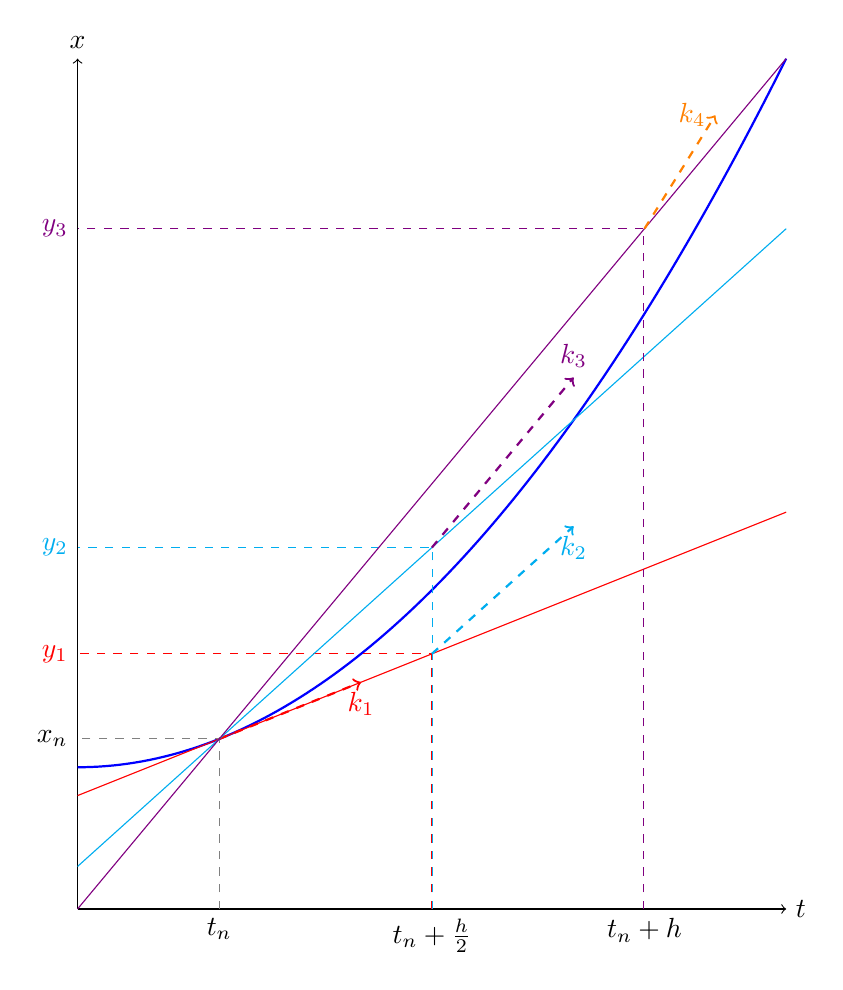
\begin{tikzpicture}[scale=0.9]
	\draw[->] (0,0) -- (10,0);
	\node[right] at (10,0) {$t$};
	\draw[->] (0,0) -- (0,12);
	\node[above] at (0,12) {$x$};
	
	\node[below] at (2,0) {$t_n$};
	\node[below] at (8,0) {$t_n+h$};
	\node[below] at (5,0) {$t_n+\frac{h}{2}$};
	
	\draw[thick,blue,domain=0:10,samples=100] plot (\x,{2+(\x*\x)/10});
	% dx/dt = x/5
	
	\draw[dashed,gray] (2,0) -- (2,2.4) -- (0,2.4);
	\node[left] at (0,2.4) {$x_n$};

	\draw[red,domain=2:4,dashed,thick,->] plot (\x, { 0.4*(\x-2)+2.4 });
	\node[below,red] at (4,3.2) {$k_1$};
	\draw[red,domain=0:10] plot (\x, { 0.4*(\x-2)+2.4 });
	\draw[red,dashed] (4.99,0) -- (4.99,3.6) -- (0,3.6);
	\node[red,left] at (0,3.6) {$y_1$};
	
	\draw[cyan,thick,dashed,domain=5:7,->] plot (\x, { 0.9*(\x-5) + 3.6 });
	\node[below,cyan] at (7,5.4) {$k_2$};
	\draw[cyan,domain=0:10] plot (\x, { 0.9*(\x-2) + 2.4 });
	\draw[cyan,dashed] (5.01,0) -- (5.01,5.1) -- (0,5.1);
	\node[left,cyan] at (0,5.1) {$y_2$};
	
	\draw[violet,domain=5:7,dashed,thick,->] plot (\x, { 1.2*(\x-5) + 5.1 });
	\node[above,violet] at (7,7.5) {$k_3$};
	\draw[violet,domain=0:10] plot (\x, { 1.2*(\x-2) + 2.4 });
	\draw[violet,dashed] (7.99,0) -- (7.99,9.6) -- (0,9.6);
	\node[violet,left] at (0,9.6) {$y_3$};
	
	\draw[thick,orange,dashed,domain=8:9,->] plot (\x, { 1.6*(\x-8) + 9.6 });
	\node[orange,left] at (9,11.2) {$k_4$};
	
	% (0.4+1.8+2.4+1.6)/6=6.2/6=1.0333 is overall gradient estimate
	

\end{tikzpicture}
\end{center}


\begin{center}
\begin{tikzpicture}[scale=0.8]
	\draw[->] (0,0) -- (10,0);
	\node[right] at (10,0) {$t$};
	\draw[->] (0,0) -- (0,12);
	\node[above] at (0,12) {$x$};
	
	\node[below] at (2,0) {$t_n$};
	\node[below] at (8,0) {$t_n+h$};
	\node[below] at (5,0) {$t_n+\frac{h}{2}$};
	
	\draw[thick,blue,domain=0:10,samples=100] plot (\x,{2+(\x*\x)/10});
	
	\draw[red,domain=0:10] plot (\x, { 1.0333*(\x-2) + 2.4 });
	\draw[dashed,red] (8,0) -- (8,8.6) -- (0,8.6);
	\node[left] at (0,8.6) {$x_{n+1}$};
	
	\draw[cyan,thick,->,domain=2:4] plot (\x, { 1.0333*(\x-2) + 2.4 });
	\node[cyan,above] at (4,4.467) {$\frac{k_1+2k_2+2k_3+k_4}{6}$};
\end{tikzpicture}
\end{center}


\clearpage




\textbf{Practice:}\bigskip


Use the classical Runge-Kutta method, RK4, to solve the following problems.

\begin{enumerate}
	\item Estimate $x(1)$ given that
		\[\deriv{x}{t} = (t+x)(t-x),\quad x(0)=3.\]
		Use a step-size of $0.2$.
	\item Estimate $y(7)$ given that
		\[\deriv{y}{x} = \sin(xy),\qquad y(5)=-2.\]
		Use a step-size of $0.25$.
\end{enumerate}

























\clearpage




{\bf Key Points to Remember:}

\vspace{5mm}

\begin{enumerate}
	\item Methods for solving ODEs numerically tend to be iterative; they take an estimate of the solution at time $t$, and a small step-size $h$, and produce an estimate of the solution at time $t+h$. Starting from the initial condition, they can then find values of the solution at later times, but errors tend to accumulate, so the larger the value of $t$ at which you want to estimate the solution, the less accurate your estimate is likely to be.
	\item \textbf{Euler's Method} works by taking the estimate $x_n$ of the solution at time $t_n$, plugging it into the ODE to estimate $x'(t_n)$, then setting $x_{n+1}=x_n+hx'(t_n)$; \textit{i.e.}, it assumes the solution has constant rate-of-change between $t_n$ and $t_n+h$. Euler's method is quick and simple, but not very accurate.
	\item \textbf{Runge-Kutta methods} are a class of methods (of which Euler's method is the simplest example) which take multiple estimates of the derivative of the solution throughout the timestep $t_n$ to $t_n+h$, and take a weighted average of these to get a better idea of the average rate-of-change $k$ of the solution between $t_n$ and $t_n+h$, and then set $x_{n+1}=x_n+hk$. The more estimates of the derivative that are taken, the longer the calculation takes, but the higher the accuracy that can be acheived.
	\item The \textbf{classical (fourth-order) Runge-Kutta method, RK4}, is a Runge-Kutta method which takes 4 estimates of the derivative and averages them, as follows:
		\begin{align*}
			k_1 &= f(t_n,x_n),\quad y_1=x_n+k_1\frac{h}{2}\\
			k_2&=f\left(t_n+\frac{h}{2},y_1\right),\quad y_2=x_n+k_2\frac{h}{2}\\
			k_3&=f\left(t_n+\frac{h}{2},y_2\right),\quad y_3=x_n+k_3h\\
			k_4&=f(t_n+h,y_3).
		\end{align*}
		Then we set $t_{n+1}=t_n+h$, and
		\[x_{n+1}=x_n + \frac{k_1+2k_2+2k_3+k_4}{6}h.\]
	\item RK4 provides a good compromise between accuracy and ease of computation. It is straightforward to implement on a computer, and widely used in the numerical solution of ODEs.
\end{enumerate}









\end{document}